\documentclass[border=6pt]{standalone}
\usepackage{tikz}
\usepackage[edges]{forest}
\usetikzlibrary{arrows.meta,positioning,calc,decorations.pathreplacing,shapes.geometric}
\begin{document}
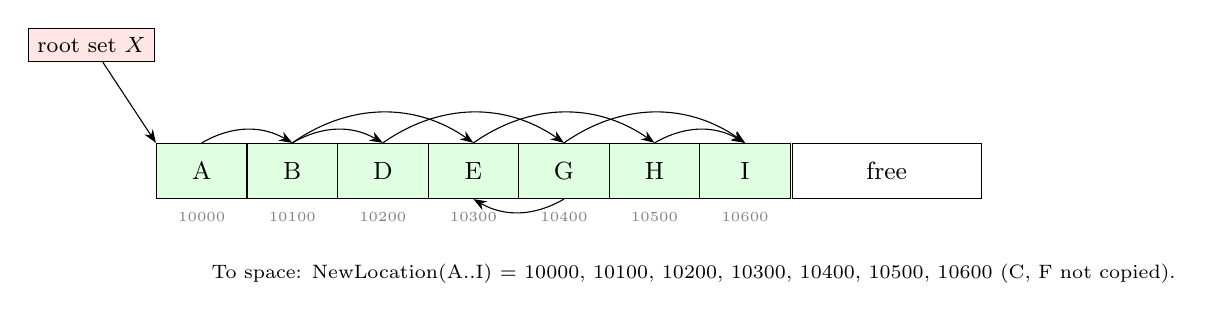
\begin{tikzpicture}[>=Stealth,font=\small]
\node[draw,minimum width=1.15cm,minimum height=0.7cm,fill=green!12] (oA) at (0.00,0) {A};
\node[font=\tiny,gray,below=0.05cm of oA] {10000};
\node[draw,minimum width=1.15cm,minimum height=0.7cm,fill=green!12] (oB) at (1.15,0) {B};
\node[font=\tiny,gray,below=0.05cm of oB] {10100};
\node[draw,minimum width=1.15cm,minimum height=0.7cm,fill=green!12] (oD) at (2.30,0) {D};
\node[font=\tiny,gray,below=0.05cm of oD] {10200};
\node[draw,minimum width=1.15cm,minimum height=0.7cm,fill=green!12] (oE) at (3.45,0) {E};
\node[font=\tiny,gray,below=0.05cm of oE] {10300};
\node[draw,minimum width=1.15cm,minimum height=0.7cm,fill=green!12] (oG) at (4.60,0) {G};
\node[font=\tiny,gray,below=0.05cm of oG] {10400};
\node[draw,minimum width=1.15cm,minimum height=0.7cm,fill=green!12] (oH) at (5.75,0) {H};
\node[font=\tiny,gray,below=0.05cm of oH] {10500};
\node[draw,minimum width=1.15cm,minimum height=0.7cm,fill=green!12] (oI) at (6.90,0) {I};
\node[font=\tiny,gray,below=0.05cm of oI] {10600};
\node[draw,minimum width=2.4cm,minimum height=0.7cm] at (8.70,0) {free};
\draw[->,black] (oA.north) to[bend left=30] (oB.north);
\draw[->,black] (oB.north) to[bend left=30] (oD.north);
\draw[->,black] (oB.north) to[bend left=35] (oE.north);
\draw[->,black] (oD.north) to[bend left=35] (oG.north);
\draw[->,black] (oE.north) to[bend left=35] (oH.north);
\draw[->,black] (oG.south) to[bend left=30] (oE.south);
\draw[->,black] (oG.north) to[bend left=35] (oI.north);
\draw[->,black] (oH.north) to[bend left=30] (oI.north);
\node[draw,fill=red!10,font=\footnotesize] (x) at (-1.4,1.6) {root set $X$};
\draw[->] (x) -- (oA.north west);
\node[font=\scriptsize,anchor=west] at (0,-1.3) {To space: NewLocation(A..I) = 10000, 10100, 10200, 10300, 10400, 10500, 10600 (C, F not copied).};
\end{tikzpicture}
\end{document}
